\section{Java Native Interface (JNI)}
\begin{figure}[thp]
\centering
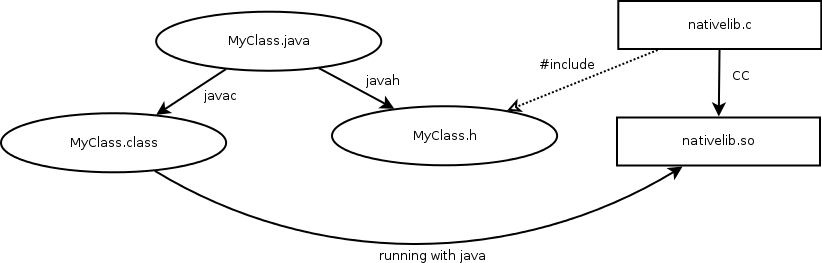
\includegraphics[scale=0.5]{img/jni/jni.png}
\caption{Passi di compilazione e di esecuzione del codice Java con l'utilizzo
dell'interfaccia JNI. Tratto da \parencite{libro:jni}.}
\label{fig:jni}
\end{figure}
La \textsc{Java Native Interface} (JNI) è utilizzata principalmente per incorporare al codice Java 
il \textit{native code} scritto con alcuni linguaggi quali il C ed il C++, e compilato
in un codice binario per il \textit{target}. Ciò implica indirettamente che
il codice prodotto non sarà più eseguibile in modalità \textit{multi-host}, rendendo
pertanto necessaria in quel caso la ricompilazione della parte dipendente 
dall'architettura del sistema. 

In questa trattazione non mi soffermerò sulle procedure di compilazione poiché 
queste sono già automatizzate dal \textit{Makefile} dell'AOSP Source\footnote{Per 
ulteriore approfondimento, queste possono essere apprese in \parencite[11-17]{libro:jni},
mentre per l'automatizzazione di questa procedura fornita dall'NDK si veda
la Sottosezione \vref{subsub:ndkbuild}.},
ma farò comunque riferimento alla strutturazione del codice per permettere una
comunicazione tramite l'interfaccia JNI: tale procedura è comunque riassunta in Figura \vref{fig:jni}.


All'interno di una classe Java possiamo specificare l'esistenza di un metodo
nativo, e quindi non implementato all'interno di tale sorgente, utilizzando
la seguente sintassi:
\begin{java}
class MyClass {
	private native void method();
	public void othermethod() {
		/* no further ancillary data is provided */
	}
}
\end{java}
Possiamo invece definire tale metodo all'interno del codice nativo nel modo che
segue:
\begin{clang}
#include <jni.h>
#include "MyClass.h"

JNIEXPORT void JNICALL Java_MyClass_method(JNIEnv *env, jobject this) {
	jclass class = (*env)->GetObjectClass(env,this);
	jmethodID callee = (*env)->GetMethodID(env,class,"othermethod"."()V");
	(*env)->CallVoidMethod(end,obj,callee);
}
\end{clang}
In particolare, il primo parametro fa riferimento ad un puntatore ad un array
ove sono contenuti tutti i metodi che è possibile chiamare da codice nativo, mentre 
il secondo è un'istanza dell'oggetto che ha invocato tale metodo.

All'interno di questo codice ho fornito un esempio di chiamata a metodo all'interno
della classe \texttt{\small MyClass} Java chiamato \texttt{\small othermethod}.
\bigskip

Tuttavia questo non è l'unico modo di effettuare transizioni all'interno della
JNI: si è per tanto in grado di creare un'istanza della \textsc{Java Virtual Machine} 
all'interno del codice nativo, allo scopo di eseguire codice Java. Un esempio
di come ciò possa essere utilizzato per eseguire metodi dichiarati nel codice Java, è fornito dalla
funzione \texttt{\small main} di inizializzazione della DVM nel Listato \vref{alg:dalvikmaincpp}.

\begin{algorithm}[thp]
\begin{cpp}[caption=$ $dalvik/dalvikvm/Main.cpp,label=alg:dalvikmaincpp]
int main(int argc, char* const argv[])
{
    JavaVM* vm = NULL;
    JNIEnv* env = NULL;
    JavaVMInitArgs initArgs;
    JavaVMOption* options = NULL;
    char* slashClass = NULL;
    int optionCount, curOpt, i, argIdx;
    int needExtra = JNI_FALSE;
    int result = 1;

    //Omissis
    /* Start VM.  The current thread becomes the main thread of the VM. */
    if (JNI_CreateJavaVM(&vm, &env, &initArgs) < 0) goto bail;

    //Omissis
    /* We want to call main() with a String array with our arguments in it.
     * Create an array and populate it.  Note argv[0] is not included. */
    jobjectArray strArray;
    strArray = createStringArray(env, &argv[argIdx+1], argc-argIdx-1);
    if (strArray == NULL) goto bail;

    /*Find [class].main(String[]).*/
    jclass startClass;
    jmethodID startMeth;

    /* Omissis: convert "com.android.Blah" to "com/android/Blah" */
    startClass = env->FindClass(slashClass);
    //Omissis
    startMeth = env->GetStaticMethodID(startClass,"main", "([Ljava/lang/String;)V");
    if (startMeth == NULL) {
        fprintf(stderr, "Dalvik VM unable to find static main(String[]) in '%s'\n",slashClass);
        goto bail;
    }

    /*Make sure the method is public.  JNI doesn't prevent us from calling
     * a private method, so we have to check it explicitly.*/
    if (!methodIsPublic(env, startClass, startMeth)) goto bail;

    /*Invoke main().*/
    env->CallStaticVoidMethod(startClass, startMeth, strArray);
    if (!env->ExceptionCheck()) result = 0;

bail:
    if (vm != NULL) {
        /* This allows join() and isAlive() on the main thread to work
         * correctly, and also provides uncaught exception handling. */
        if (vm->DetachCurrentThread() != JNI_OK) {
         fprintf(stderr, "Warning: unable to detach main thread\n"); result = 1;
        }
        if (vm->DestroyJavaVM() != 0)
            fprintf(stderr, "Warning: Dalvik VM did not shut down cleanly\n");
    }
    //Omissis
}
\end{cpp}
\end{algorithm}



\subsection{Esempi di interazione tra AOSP Source e Kernel Android}
\subsubsection{UEventObserver}
Fornisco ora un esempio piuttosto immediato per mostrare come, tramite l'utilizzo della JNI, sia possibile intercettare direttamente all'interno di codice Java, del tutto indipendente dall'architettura della macchina, eventi sollevati dallo stesso Kernel. La classe \texttt{\small UEventObserver} di fatti costituisce un ponte tra i servizi offerti dall'AOSP ed eventi sollevati dal Kernel: utilizzando infatti la libreria \textit{libhardware\_legacy}, è in grado di raccogliere gli eventi generati dall'interazione dell'utente con il dispositivo, tramite l'accesso alla \textit{systemcall} \texttt{\small socket} come mostrato dal file:
\begin{center}
\AOSP\texttt{\small/hardware/libhardware\_legacy/uevent/uevent.c}
\end{center}
In particolare si ascolterebbero gli eventi Netlink nel seguente modo:
\begin{clang}
socket(PF_NETLINK,SOCK_DGRAM,NETLINK_KOBJECT_UEVENT)
\end{clang}
Questo mostra in parte come alcune interazioni non vengono gestite unicamente dal Kernel, ma di come spesso il comportamento di base sia modificato dalle funzioni definite in Java, come nell'esempio.

\subsubsection{Binder}
Un ulteriore esempio di come si utilizzi JNI all'interno di Android è
fornito dal Binder (v. Sezione \vref{sec:ipcbinder}): come si può evincere 
dal sorgente,  anche questo meccanismo
sia implementato su più livelli:
\begin{description}
\item[Definizione di interfaccia API] Si provvedono tra le altre le interfacce\\
	\texttt{\small android.os.Parcelable} e \texttt{\small android.os.IBinder},
	e le classi \texttt{\small android.os.Parcel}, \texttt{\small android.os.Bundle},
	\texttt{\small android.content.Intent} e \texttt{\small android.os.Binder}
\item[JNI] Anche in questo caso si utilizza del codice C++ per effettuare 
	il collegamento tra l'implementazione in C++ e le API Java: tale \textit{bridge}
	è fornito dal file:
	\begin{center}
	\texttt{\small \AOSP/frameworks/base/core/jni/android\_util\_Binder.cpp}
	\end{center}
\item[C++ ``middleware''] Questo ulteriore strato di codice si frappone
	tra il driver di sistema immediatamente sottostante ed il livello delle
	JNI, creando l'implementazione delle primitive di comunicazione. I 
	sorgenti di questo livello architetturale sono forniti all'interno
	del percorso:
	\begin{center}
	\texttt{\small \AOSP/frameworks/native/libs/binder/}\footnote{Il posizionamento
	di tali sorgenti è stata cambiata dalla redazione di  \parencite{tesi:binder},
	dove questi erano localizzati in  \texttt{\small \AOSP/frameworks/base/libs/utils/}.

	Analogamente vale per lo stato di Kernel Driver, dove in quei tempi tale
	implementazione era localizzata in \texttt{\small \AOSP/drivers/staging/android/}.
	}
	\end{center}
\item[Kernel Driver] Il file:
	\begin{center}
	\texttt{\small ./frameworks/base/cmds/servicemanager/binder.c}
	\end{center}
	fornisce un'implementazione sulle \textit{systemcall} sulle operazioni di
	\texttt{\small open}, \texttt{\small mmap}, \texttt{\small release}, \texttt{\small poll}
	e \texttt{\small ioctl}.
\end{description}

Questa trattazione preliminare mostra come la descrizione fornita dalla Figura \vref{fig:androidsourceView}
possa descrivere solamente come, in prima battuta, si presenti il Binder a 
livello di applicazioni Java: in realtà anche il Binder si dispone sia a livello
di \textit{Android Framework Libraries}, sia a livello di \textit{Native Libs}, sia
a livello \textit{Android Kernel} predisponendo un driver.
\medskip

Un'ulteriore esempio di implementazione di servizio lato Java dal quale poi
ricevere le richieste lato Java è fornito da \parencite{site:marakRemixing}.
Tuttavia nel sorgente proposto non sono ancora previste \textit{upsyscall} 
da programmi C.
